\documentclass[11pt]{article}
\usepackage{graphicx}
\usepackage{hyperref}
\usepackage{amsmath}
\usepackage{caption}
\usepackage{float}
\usepackage{geometry}
\geometry{margin=1in}

\title{Analysis of Average Waiting Time in a Producer-Consumer System}
\author{Rousomanis Georgios (10703)}
\date{May 2025}

\begin{document}

\maketitle

\section{Introduction}

The producer-consumer problem is a classic example of a multi-thread synchronization issue, 
where multiple producer threads generate data and insert it into a shared queue, and multiple 
consumer threads remove and process this data. In this report, we analyze the behavior of such 
a system, focusing on the average waiting time of items in the queue, defined as the duration 
between the time an item is enqueued by a producer and the time it is dequeued by a consumer.

\section{Experimental Setup}

The experiment was performed on a 4-core machine using a custom implementation of the 
producer-consumer pattern written in C, utilizing POSIX threads (pthreads). The system includes:
\begin{itemize}
    \item A fixed-size FIFO queue of size 10.
    \item Each producer performs 10,000 iterations of adding dummy work to the queue.
    \item Consumers retrieve and immediately process this work.
    \item No artificial delays (e.g., \texttt{sleep()} or \texttt{usleep()}) are introduced in 
    either producers or consumers.
    \item The average waiting time is measured for each item from the moment it is enqueued until 
    it is dequeued.
\end{itemize}

The main variable parameters are:
\begin{itemize}
    \item \( P \in \{1, 2, 4, 8\} \): the number of producer threads.
    \item \( Q \in [1, 20] \): the number of consumer threads.
\end{itemize}

\section{Results and Discussion}

Figure~\ref{fig:avg_waiting_time} presents the average waiting time (in microseconds) as a function 
of the number of consumer threads \( Q \), for different values of producer threads \( P \).

\begin{figure}[H]
    \centering
    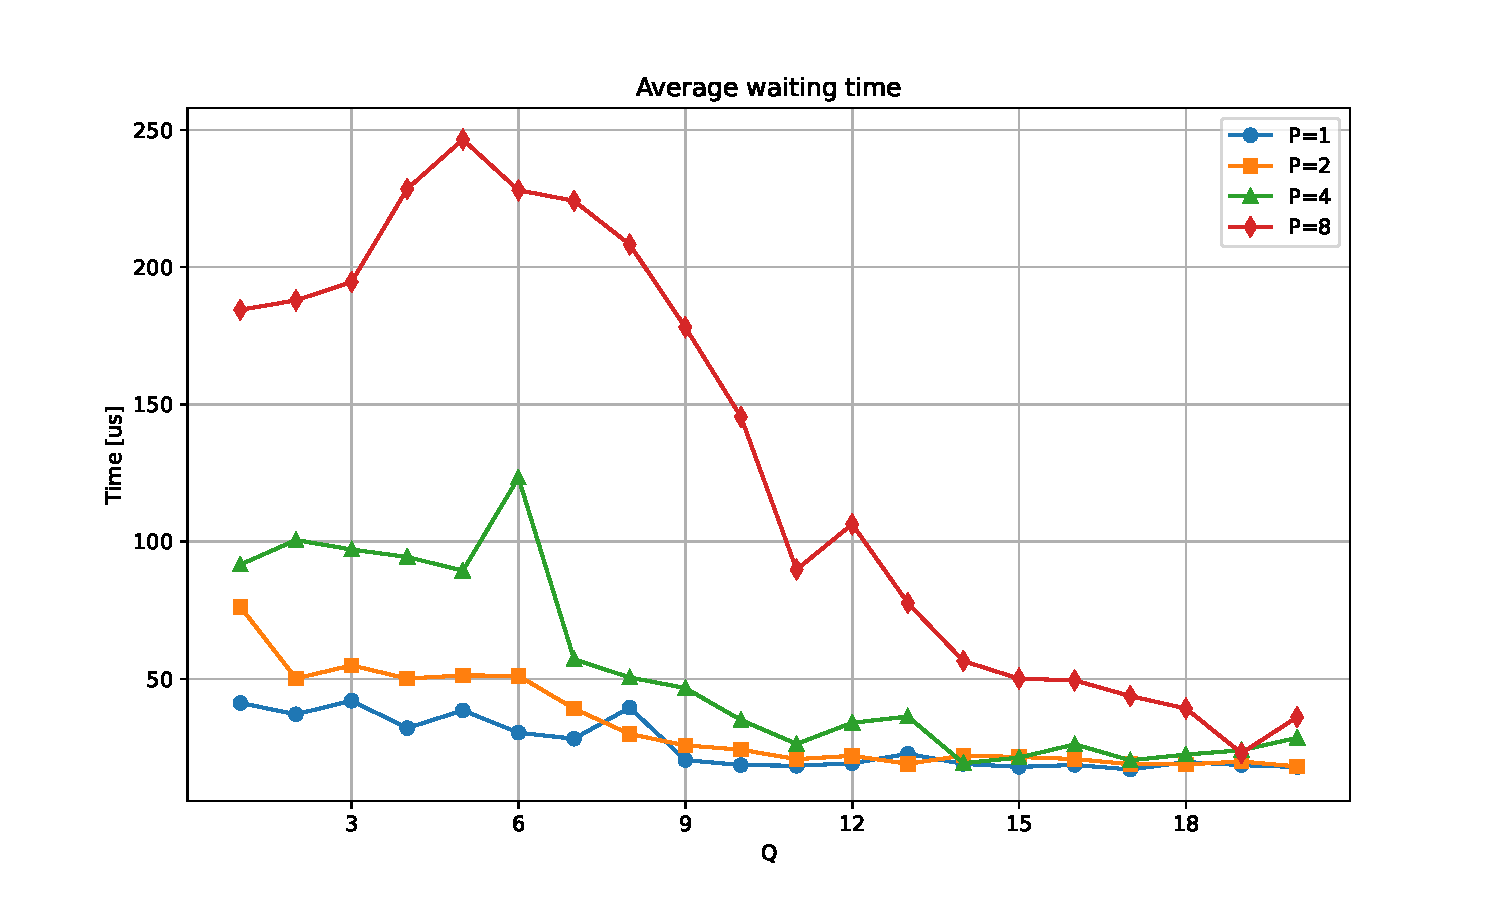
\includegraphics[width=0.85\textwidth]{figure.pdf}
    \caption{Average waiting time vs. number of consumer threads \( Q \), for various values of \( P \).}
    \label{fig:avg_waiting_time}
\end{figure}

The observed trends can be summarized as follows:
\begin{itemize}
    \item For a small number of consumer threads, the queue tends to fill up quickly, causing producer 
    threads to block and resulting in higher waiting times.
    \item As \( Q \) increases, consumers are able to process items more promptly, decreasing the 
    average waiting time.
    \item When \( Q \) becomes sufficiently large, the waiting time decreases sharply and then tends 
    to plateau, indicating that adding more consumers yields diminishing returns.
    \item Higher values of \( P \) consistently result in higher waiting times for the same \( Q \), 
    due to increased contention for the shared queue.
\end{itemize}

Notably, for \( P = 8 \), the system becomes significantly more congested, especially when \( Q \) is low. 
This reflects a situation where production outpaces consumption, causing the queue to reach capacity more 
frequently and introducing delays for both producers and consumers.

\section{Conclusion}

The experiment highlights the importance of balancing producer and consumer threads in a multi-threaded system. 
Under-provisioned consumer capacity leads to longer waiting times and reduced system responsiveness. On a 4-core 
system, optimal performance is generally achieved when the number of threads is aligned with the hardware's 
parallel capabilities. For compute-light workloads such as this one (dummy work), consumer saturation occurs 
quickly, and additional threads do not substantially improve throughput.

These insights are essential for designing concurrent applications that require efficient inter-thread communication, 
especially under real-time constraints.

\begin{itemize}
    \item Producer-consumer problem source code: 
    
    \url{https://github.com/georrous6/Real-Time-Embedded-Systems.git}
    \item K-nearest neighbors source code: 
    
    \url{https://github.com/georrous6/Parallel-and-Distributed-Systems.git}
\end{itemize}

\end{document}

